\chapter{Ambiernte de Desenvolvimento}

\section{Ambiente de Aplicação}

Existem basicamente dois tipo de ambiente que os quadrotores aéreos podem atuar: o ambiente indoor e o ambiente outdoor. Nas missões em ambiente outdoor os quadrotores são expostos a ambientes desconhecidos, onde existe a forte presença de pertubações, como rajadas de vento e obstáculos dinâmicos. Nesse tipo de missão, os quadrotores muitas vezes vão precisar de sensores do tipo GPS para ajudar na localização do veículo e também, um controlador adequado para lidar com a rejeição de pertubação e com as incertezas paramétricas, além de um planejador de trajetória online. As missões indoor possuem menos pertubações e ambientes mais estruturados. Sendo possível fazer o mapeamento prévio do ambiente para realizar as operações.

\section{Situação Atual do Desenvolvimento}

As pesquisas mais atuais na área se concentram em áreas como controle, planejamento de trajetória, autonomia, percepção e navegação autônoma. O controle ainda é muito estudado pelo fato desse tipo de aeronave ser naturalmente instável, não-linear e subatuada, sendo necessário o desenvolvilmento de controladores eficientes para realizar o segmento de trajetória, a rejeição de pertubação e ter insensibilidade a erros de modelagem e de incertezas paramétricas de forma ótima, com o menor gasto energético. O planejamento de trajetória também é desafiador pelo fato do ambiente de atuação ser tridimensional, que aumenta muito o custo computacional dos algoritmos. Isso torna necessário o estudo de algortimos otimizados, com custos computacionais menores, permitindo que o planejador calcule trajetórias em tempos inferiores. Na questão de autonomia, uma grande limitação dos veículos aéreos de asas rotativas de forma geral é o gasto energético que a aeronave tem para manter vôo. Utilizar baterias maiores aumenta também o peso da aeronave, sendo necessário o estudo das melhores tecnlogias que vem sendo usadas. Tem surgido pesquisas também de recarregamento desse tipo de aeronave wireless em estações preparadas para isso.

\section{Mercado de Atuação}

Os quadrotores são muito utilizados tanto em aplicações civís como em aplicações militares. Em aplicações militares, pelo fato desse tipo de aeronave possuir alta manobrabilidade e possibilidade de vôo estacionários ou quase estacionários, eles podem ser utilizados em missões de espionagem, monitoramento e vigilância. Como elas não necessitam de um piloto embarcado, não o colocando em risco, e também podem ser muito pequenas, podem ser utilizadas em missão de busca e regaste em ambientes hostís, como em situações de desmoronamento. Na área civíl, estas aeronaves tem se popularizado no seu uso para entertenimento de forma geral. Tem sido muito utilizadas na área cinematográfica para realização de vídeos e fotagrafias aéreas. Seu uso tem se popularizado também na agricultura, para realizar o monitoramento de plantações, irrigação e pulverização agrícola. Já tem sido feito o uso de quadrotores para realizar entregas delivery e também transporte aéreo de pessoas.

O uso do veículos aéreos não tripulados do tipo quadrotor tem se expandido em diversas áreas, tanto civíl, quanto militar e também acadêmica.

No ambiente acadêmico, os quadrotores são utilziados como plataforma para teste de estratégias de controle, dada a dificuldade de se estabilizar e de controlar esse tipo de veículo, e também para teste de técnicas de planejamento de trajetória, por se deslocar no espaço tridimensional.

Os quadrotores por não necessitarem de um piloto embarcado, poderem ser pequenos e ágeis podem ser utilizados em missões de busca e resgate em abientes hostis, como casos de desmoronamento ou soterramento, e também em missões de espionagem e vigilância, por chamaerem pouca atenção.

Tem-se crescido muito o uso de aeronaves do tipo quadrotor na área de agricultura de precisão. Os drones podem ser utilizados para monitorar uma lavroura, mapear, distribuir uso de defensivos, semear e até mesmo irrigar.

Outra área de grande utilização é a de enterterimento. Existem muitos drones são comercializados com finalidade exclusivamente lúdica, podendo ser equipados com câmeras para produzir fotografias e vídeos. São utilizados tambpem na cinematografia para realizar essas filmagnes aéreas, que antes eram feitas por helicópteros tripulados que tinham custo associados muito maiores.

\chapter{Metodologia}
\label{chap:metodologia}
%--------- NEW SECTION ----------------------
A pesquisa do estudo do estado da arte desenolvido neste documento foi elaborada principalmente a partir do método BILI, que permite realizar uma pesquisa bibliográfica em um banco de dados de artigos científicos, publicações em periódicos, livros e outras fontes de conhecimento científicos, fazendo o levantamento das publicações e dos autores mais impactantes na área pesquisada. Também foram realizadas pesquisas para avaliar as soluções encontradas já no mercado.

O método BILI é dívidido em quatro ciclos que acontecem em sequência. Eles são chamados de ciclo ingênuo, ciclo otimizada, ciclo de impacto e ciclo de produção.

% BIBLIOMETRIX


\begin{figure} [h!]	
  \centering
  \caption{Método BILI}
  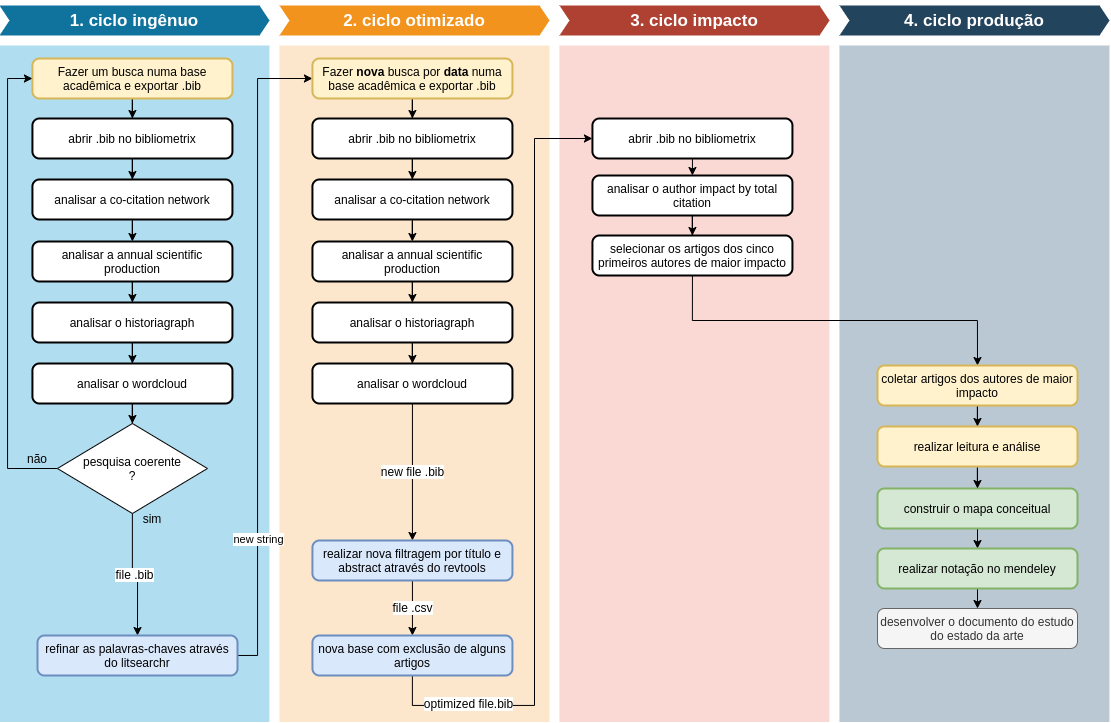
\includegraphics[width=1\textwidth]{Figures/bili.png}
  \caption*{Fonte: Autoria própria.}
  \label{fig:QFD}
\end{figure}

\section{Ciclo Ingênuo}
No primeiro ciclo do método BILI é feita uma busca das pesquisas desenvolvidas na área estudada em um banco de dados de documentos acadêmicos, através de palavras-chave que tenham conexão o tema proposto. O banco de dados escolhido para aplicar o método foi o Scopus.

O resultado da busca no banco de dados com as palavras-chave é um arquivo .bib, que contém o nome dos documentos encontrados, palavras-chave, ano de publicação, nome dos autores, DOI, resumo, entre outros.

Em seguida o arquivo .bib gerado no banco de dados é aberto no Bibliometrix, que é um pacote desenvolvido para R que permite uma clara visualização das informações levantadas e também realiza análises dos dados obtido. 

É então realizada a análise da rede de cocitação, que é um gráfico que relaciona os autores, mostrando a proximidade da pesquisa realizada por eles através de citações realizadas nas pesquisas. O resultado dessa análise é positivo se a rede de cocitação estiver coesa, com todos elementos conectados.

É avaliada também a produção científica anual, que é um gráfico que mostra quantas pesquisas foram realizadas na área pesquisada ao longo do tempo. O resultado desse gráfico é coerente quando se tem um crescimento positivo do número de pesquisas realizadas com o passar do tempo.

São avaliados por último os gráficos de histograph e wordcloud, que dão idéia das pesquisas mais importantes realizadas ao longo do tempo e das palavras chaves mais utilizadas, respectivamente.

Se a pesquisa não apresentar resultados coerentes, é realizada uma nova pesquisa com palavras-chave diferentes. Caso seja coerente, o próximo passo é fazer um refinamento das palavras-chave através do litsearchr, que é um pacote desenvolvido para R, que através do arquivo .bib obtido, fornece as palavras-chave mais impactantes dos dados.

\section{Ciclo Otimizado}
Com as palavras-chave otimizadas obtidas através do litsearchr, é feita uma nova busca no banco de dados acadêmico escolhido, no caso o Scopus, para obter um novo arquivo .bib, da mesma forma que foi obtido no primeiro ciclo.

Os gráfico de rede de cocitação, produção científica anual, wordcloud e histograph são analisados novamente, para avaliar a coerência. Caso verificada a coerência do resultado, é realizada uma filtragem dos resultados através do revtools. O revtools é um pacote desenvolvido também para R onde é possível realizar a leitura do resumos das pesquisas e é possível manter a pesquisa caso ela seja útil ou excluir caso ela não sirva.

O resultado do revtools é um arquivo .csv contendo apenas os documentos que são úteis para a pesquisa. O arquivo então é convertido novamente para o formato .bib e então passado para o próximo ciclo.

\section{Ciclo de Impacto}
O arquivo .bib gerado no ciclo anterior é novamente aberto no Bibliometrix. Nessa etapa é avaliados o gráfico de author impact by total citation e levantados de três a cinco autores com maior impacto apresentados no gráfico.

\section{Ciclo de Produção}
Por último são coletados os artigos dos autores selecionados no banco de dados e é feita a leitura completa dos artigos. 

É feito o upload dos artigos e leitura na plataforma Mendeley. Nesse aplicativo é possível compartilhar os artigos com grupos de estudo e também fazer anotações e grifar trechos importantes. 

A partir dos conhecimentos adquiridos é feito um mapa conceitual que relaciona os principais conceitos apresentados para servir de base para o desenvolvimento desse documento.

%----------------------------------------------------------

%--------- NEW SECTION ----------------------


%---------------picture------------------------------------
% \begin{figure}
%     \centering
%     \subfigure[Figure A]{\label{fig:a}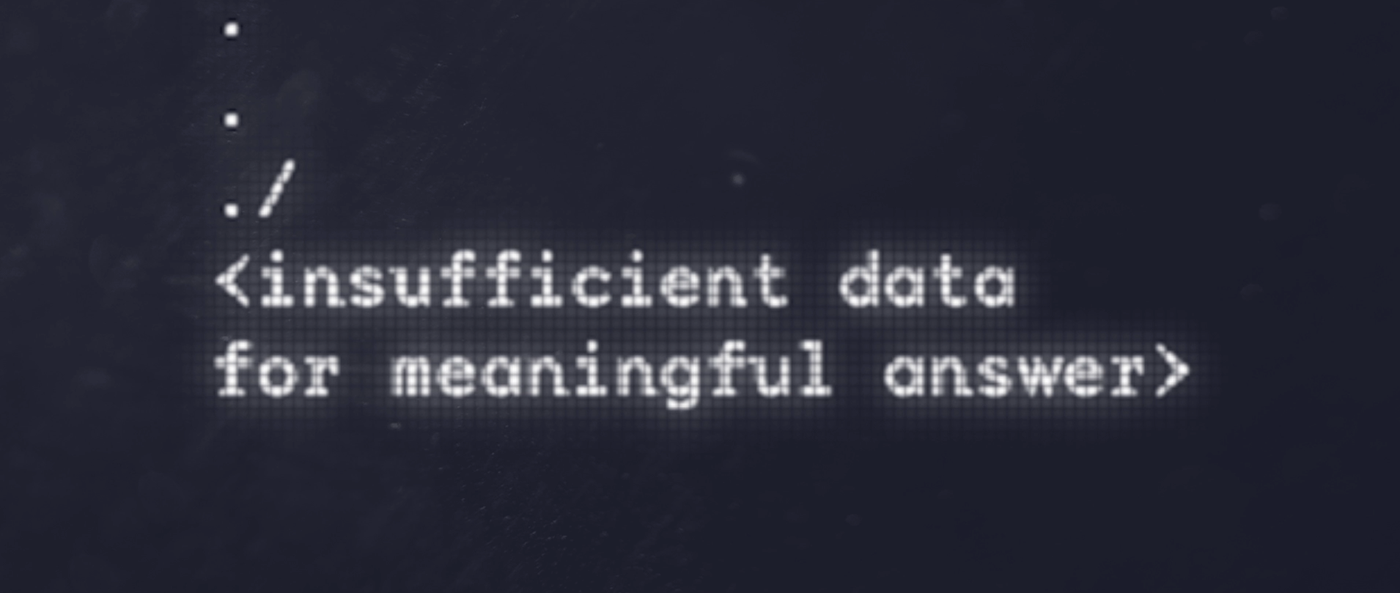
\includegraphics[width=60mm]{./lq}}
%     \subfigure[Figure B]{\label{fig:b}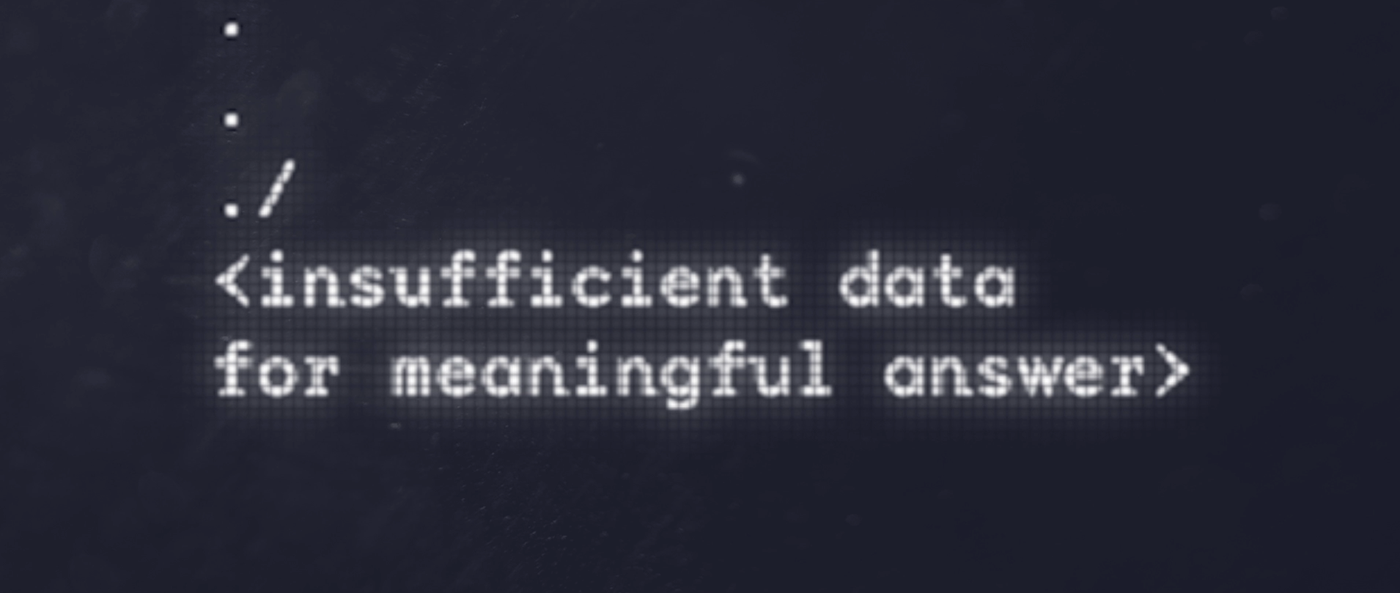
\includegraphics[width=60mm]{./lq}}
%     \subfigure[Figure C]{\label{fig:c}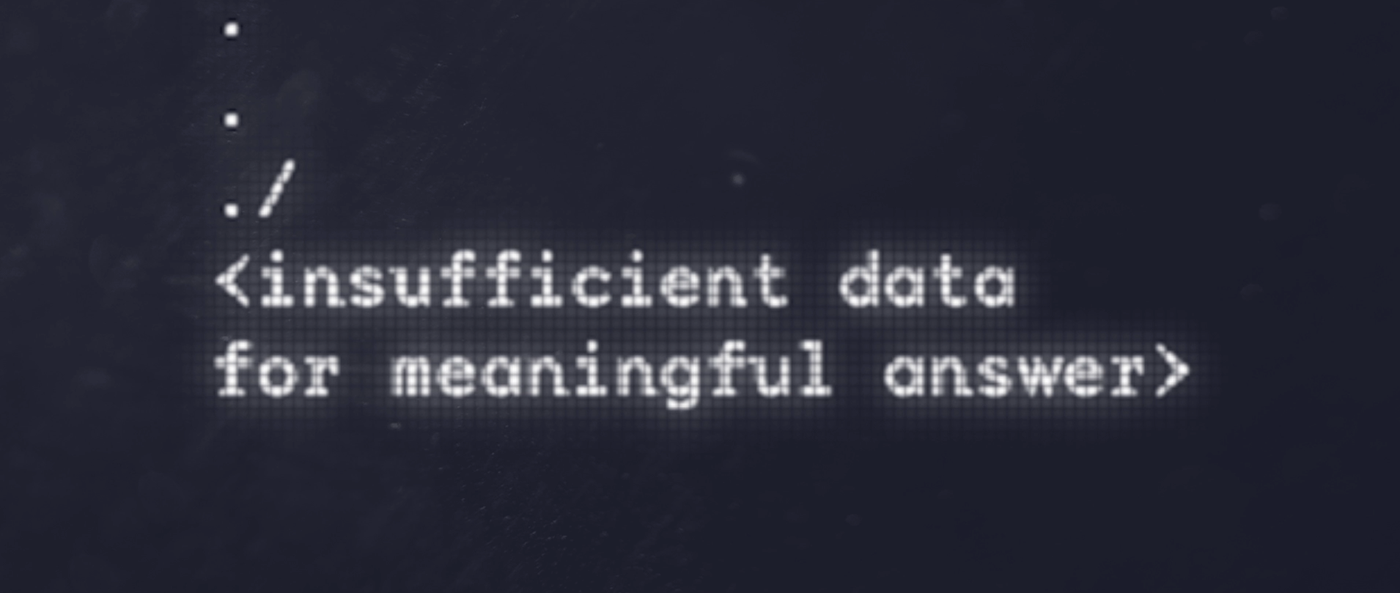
\includegraphics[width=\textwidth]{./lq}}
%     \caption{Three simple graphs}
%     \label{fig:three graphs}
% \end{figure}
%----------------------------------------------------------

% \begin{figure}
%     \centering
%     \begin{subfigure}[b]{0.3\textwidth}
%         \centering
%         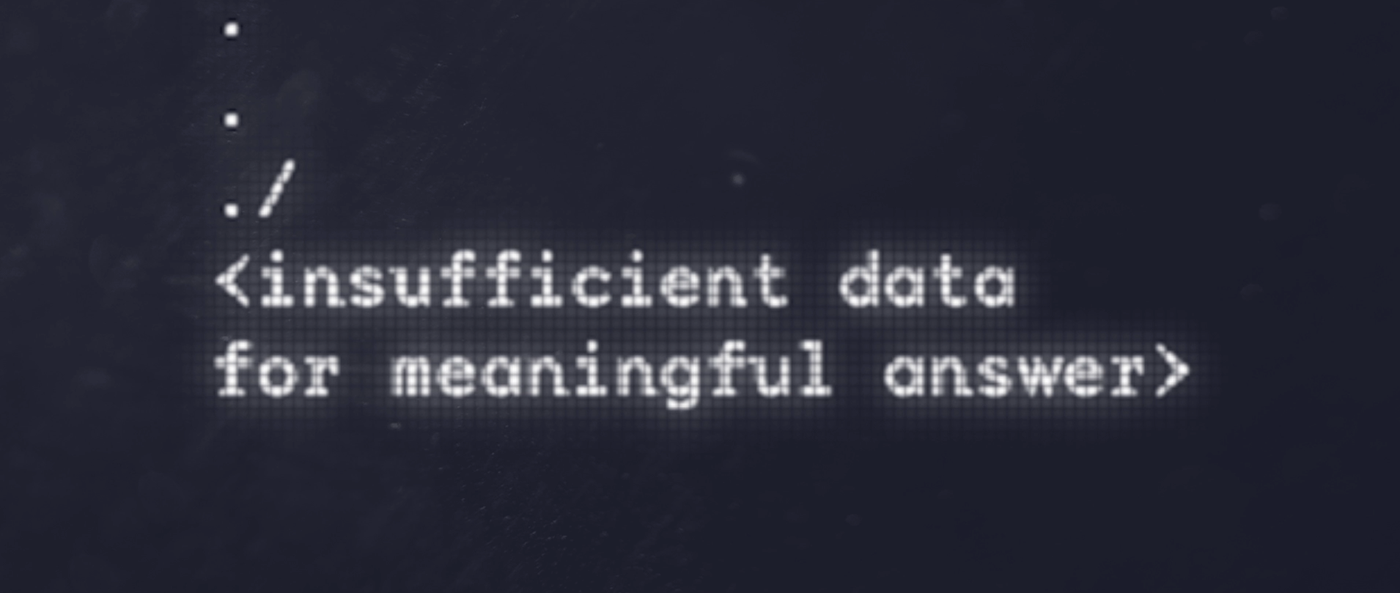
\includegraphics[width=\textwidth]{./lq}
%         \caption{$y=x$}
%         \label{fig:y equals x}
%     \end{subfigure}
%     \hfill
%     \begin{subfigure}[b]{0.3\textwidth}
%         \centering
%         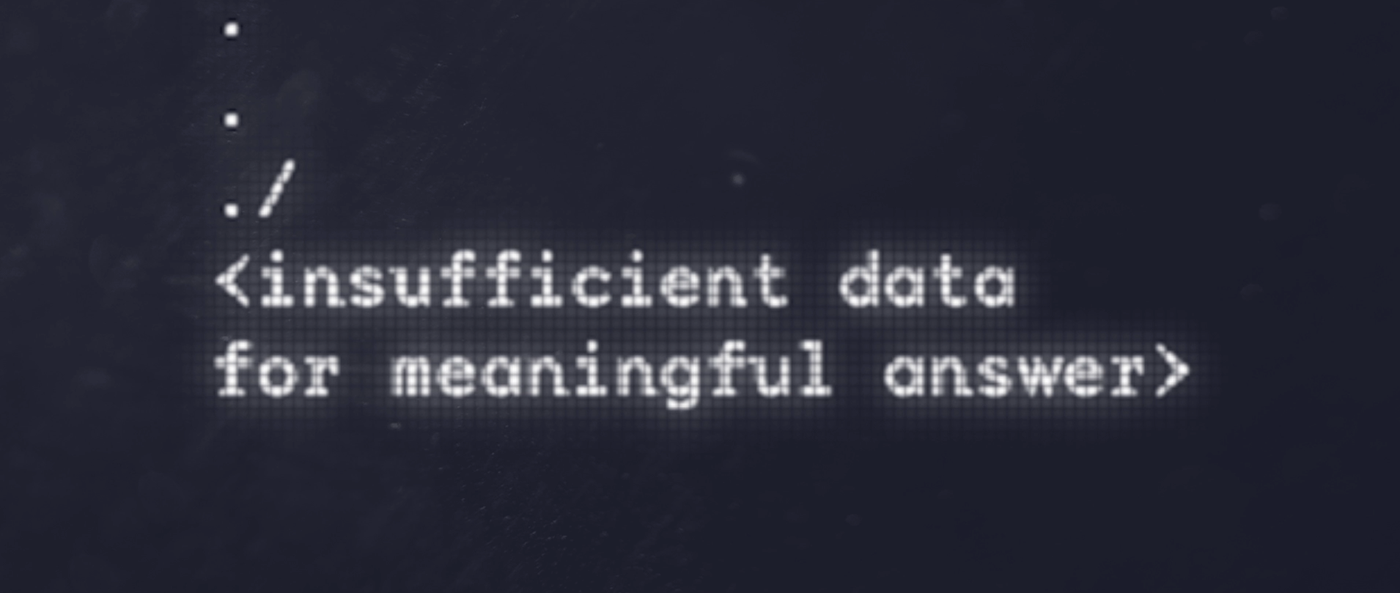
\includegraphics[width=\textwidth]{./lq}
%         \caption{$y=3sinx$}
%         \label{fig:three sin x}
%     \end{subfigure}
%     \hfill
%     \begin{subfigure}[b]{0.3\textwidth}
%         \centering
%         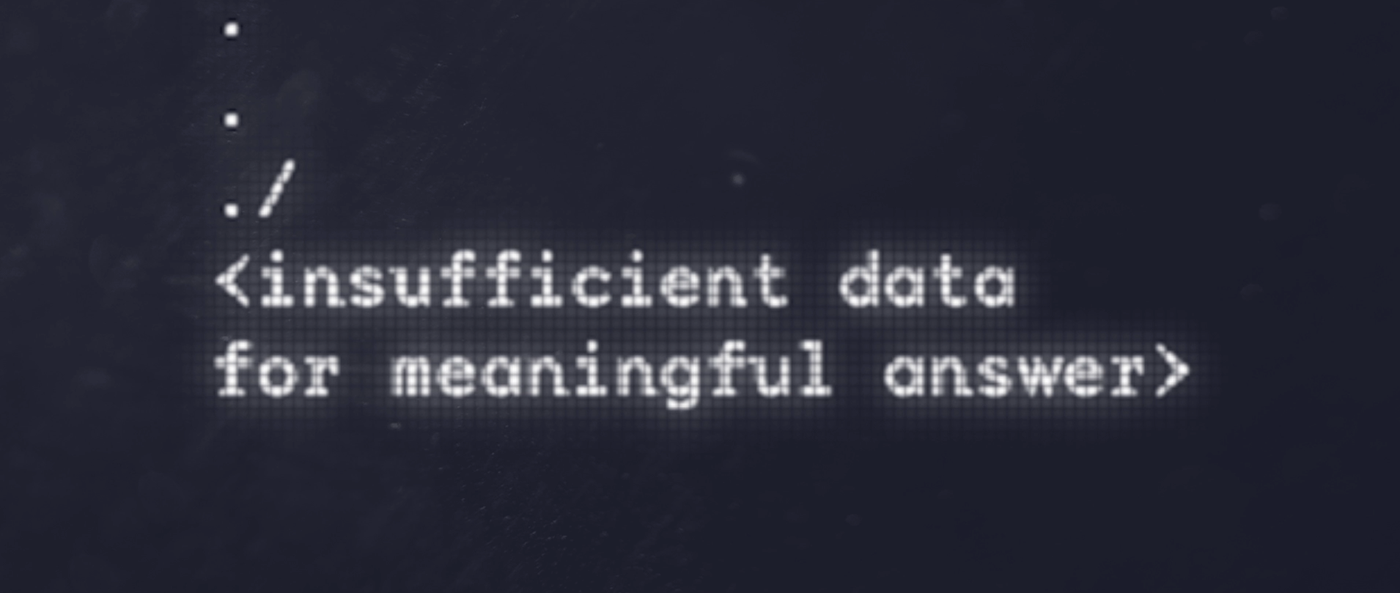
\includegraphics[width=\textwidth]{./lq}
%         \caption{$y=5/x$}
%         \label{fig:five over x}
%     \end{subfigure}
%        \caption{Three simple graphs}
%        \label{fig:three graphs}
% \end{figure}


%--------- NEW SECTION ----------------------
% \section{Assunto 2}
% \label{sec:ass2}
% flkjasdlkfjasdlkfjs

% \begin{table}[h]
%     \begin{subtable}[h]{0.45\textwidth}
%         \centering
%         \begin{tabular}{l | l | l}
%         Day & Max Temp & Min Temp \\
%         \hline \hline
%         Mon & 20 & 13\\
%         Tue & 22 & 14\\
%         Wed & 23 & 12\\
%         Thurs & 25 & 13\\
%         Fri & 18 & 7\\
%         Sat & 15 & 13\\
%         Sun & 20 & 13
%        \end{tabular}
%        \caption{First Week}
%        \label{tab:week1}
%     \end{subtable}
%     \hfill
%     \begin{subtable}[h]{0.45\textwidth}
%         \centering
%         \begin{tabular}{l | l | l}
%         Day & Max Temp & Min Temp \\
%         \hline \hline
%         Mon & 17 & 11\\
%         Tue & 16 & 10\\
%         Wed & 14 & 8\\
%         Thurs & 12 & 5\\
%         Fri & 15 & 7\\
%         Sat & 16 & 12\\
%         Sun & 15 & 9
%         \end{tabular}
%         \caption{Second Week}
%         \label{tab:week2}
%      \end{subtable}
%      \caption{Max and min temps recorded in the first two weeks of July}
%      \label{tab:temps}
% \end{table}